\chapter{Etat de l'art}
\label{chap:premierchapitre}

Dans cette section de ce mémoire, nous allons tout d'abord présenter les éléments existants permettant à partir d'exigences fonctionnelles de procéder aux tests d'acception. Nous présenterons les outils qui existent sur le marché qui tentent d'automatiser ce processus. Puis dans une seconde partie nous présenterons les différentes façons de modéliser des exigences fonctionnelles de sorte à pouvoir générer des tests d'acceptation. Enfin dans la dernière partie de ce chapitre nous proposerons, compte tenu des éléments précédemment présentés, une ébauche de solution à notre problématique que nous présenterons plus en détail dans le second chapitre de ce document.

\section{Workflow général et Critères de comparaison}

Les modèles de gestion de projets les plus répandus sont le cycle en V et la méthode agile scrum. Dans ces modèles, le besoin est recueilli, les exigences sont définies, vérifiées et testées. Dans le cycle en V schématisé dans la figure \ref{fig:cylce}, nous nous intéressons aux phases \textbf{Analyse des besoins}, \textbf{Spécifications}, \textbf{Recette} et \textbf{Test de validation}. Dans la méthode agile scrum, nous nous intéressons au contenu du product backlog, au contenu du sprint backlog et des user stories car ces étapes représentent \textbf{la définition des exigences et les tests à réaliser à la fin de chaque sprint}. En combinant les deux méthodes et en ne ciblant que les phases projet qui nous intéressent, à savoir \textbf{les phases d'analyse et de test}, nous proposons de considérer comme workflow génériques, celui du cycle en V et de la méthode Scrum.

\begin{figure}[H]
    \centering
    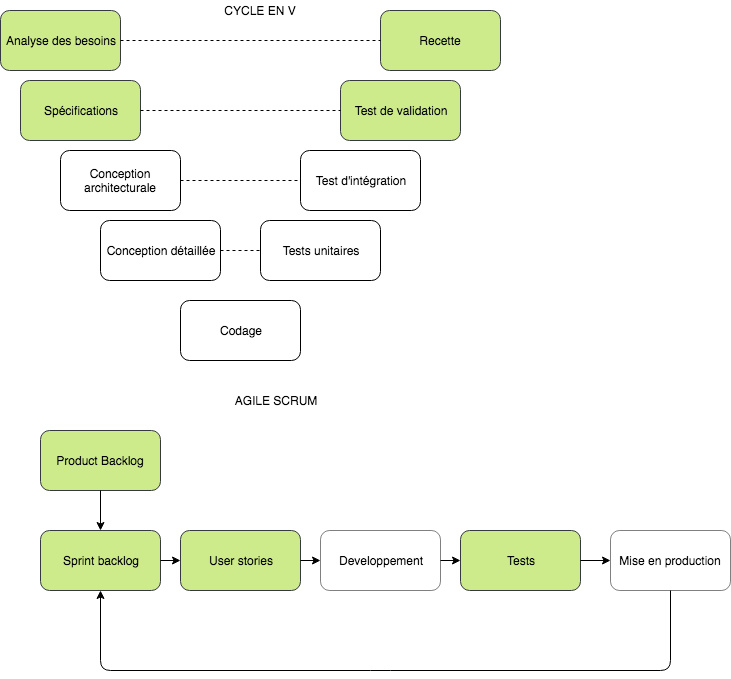
\includegraphics[width=\textwidth]{images/cycles.png}
    \caption{Phases ciblées dans ce mémoire}
    \label{fig:cylce}
\end{figure}

Dans cet état de l'art, nous comparerons et analyserons les différents outils et méthodes qui répondent entièrement ou partiellement à notre problématique selon les critères suivants :

\begin{center}
 \begin{tabular}{||c||} 
 \hline
Description des critères de comparaison \\ [0.5ex] 
 \hline\hline
Les exigences peuvent être écrites par n’importe quelle partie prenante \\ 
 \hline
Les exigences peuvent être lues par n’importe quelle partie prenante\\
 \hline
Les spécificités fonctionnelles du domaine peuvent être correctement exprimées \\
 \hline
Les exigences sont exprimées de façon à pouvoir générer des tests clairs \\
 \hline
Il existe un moyen d’automatiser les tests\\ 
 \hline
 Les tests automatisables sont des tests d’acceptation\\ 
\hline 
 Le resultat des tests est disponible au niveau des exigences\\ [1ex]
\hline 
\end{tabular}
\end{center}

\section{Présentation de l'existant}

    \subsection{Processus}
        \subsubsection{Des exigences aux tests}
        Il existe plusieurs outils sur le marché qui permettent aux clients de renseigner les tests d’acceptation à dérouler ainsi que les résultats attendus pour satisfaire les exigences. Parmi ces outils, HP ALM (Application Lifecycle Management) anciennement Quality Center. Il existe d’autres outils relativement similaire à HP ALM mais nous décidons de présenter celui-ci car nous avons récemment eu l’occasion de travailler avec au sein de Capgemini pour un client.
        
        \paragraph{HP Application Lifecycle Management (ALM)} \protect
        
        Cet outil permet la collaboration des différentes parties prenantes. En effet, les chefs de projets peuvent planifier le projet en déterminant le nombre le périmètre de cycles de releases, la spécification des exigences est également réalisée par les business analystes, les testeurs peuvent dérouler les tests, etc. Tout ceci permet d'avoir une vision globale du projet. La figure \ref{fig:hp} représente une instance des parties que nous avons ciblées du cycle en V. 
        
         \begin{figure}[H]
                \centering
                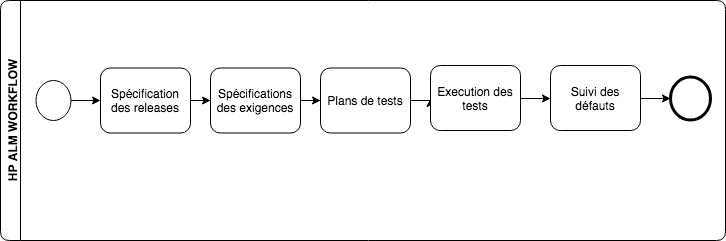
\includegraphics[width=\textwidth]{images/hpworkflowbpmn.png}
                \caption{Workflow BPMN de HP ALM}
                \label{fig:hp}
            \end{figure}
        
        La rédaction des exigences et des plans de tests se fait manuellement, en langage naturel. Les personnes en charge de dérouler les plans de test lisent les différentes étapes, les exécutent et comparent les résultats obtenus aux résultats attendus.
        
            \begin{figure}[H]
                \centering
                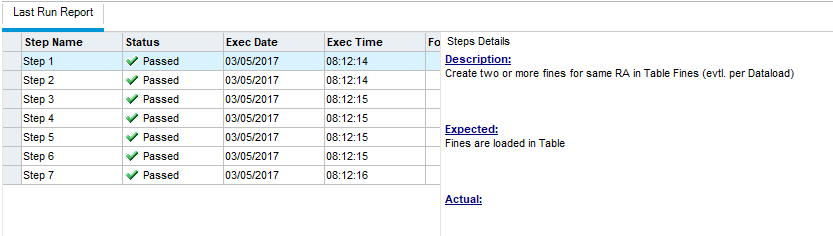
\includegraphics[width=\textwidth]{images/qc.png}
                \caption{Exemple d'un rapport de run de tests d'un projet sur lequel nous avons travaillé}
            \end{figure}
        
        Lorsqu’un comportement anormale est détecté pendant les tests, un "defect" est créé pour tracker le défaut de l’application.
        
        Bien que ce type d’outil permette d’avoir une visibilité entre les exigences et le résultat des tests il n’en reste pas moins qu’il n’existe pas d’automatisation des tests à partir des exigences.
        
        \paragraph{Framework For Integrated Test (FIT)}
        
        Des frameworks comme FitNess\cite{fitnesse} basés sur FIT (Framework For Integrated Test) tentent de répondre à la problématique de l’automatisation des tests à partir des exigences. FIT est un moteur qui traite chaque table qui représente les exigences en utilisant le code fixture à laquelle la table correspond.\textit{\guillemotleft Une fixture est un morceau de code qui permet de fixer un environnement logiciel pour exécuter des tests logiciels. Cet environnement constant est toujours le même à chaque exécution des tests. Il permet de répéter les tests indéfiniment et d'avoir toujours les mêmes résultats~\cite{fixture}.\guillemotright} Le framework Fitness permet d'afficher les résultats de ces derniers. Les tests FIT sont donc des représentations tabulaires des exigences. A partir de ces tables, des tests sont générés~\cite{article6}.Les attentes des clients sont comparés aux résultats réels.~\cite{fitnesse}

            \begin{figure}[H]
                \centering
                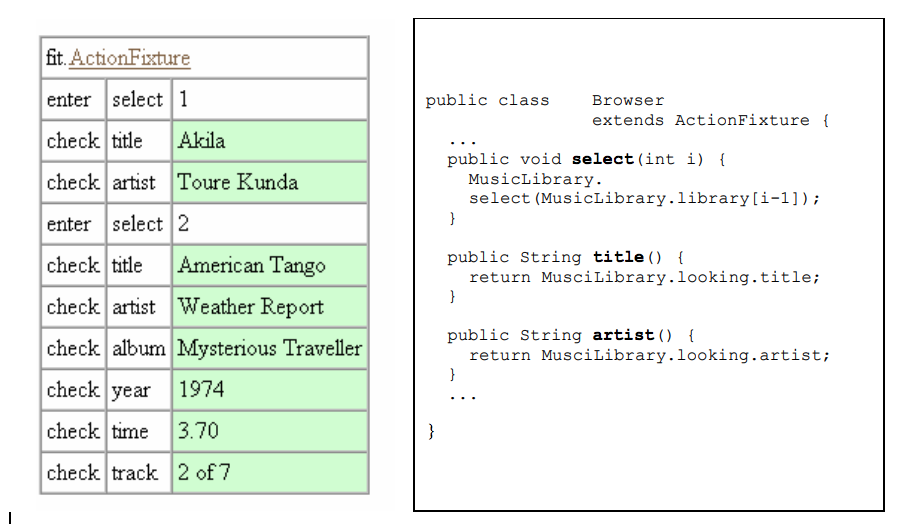
\includegraphics[width=\textwidth]{images/FIT.png}
                \caption{Exemple d'une table FIT et de la fixture générée}
            \end{figure}

        FitNess permet d'écrire et de lire les exigences de façon simplifiée mais pas simple. Les tests sont facilement mis en oeuvre par les développeurs d'après l'article~\cite{article6}. Cependant \textit{\guillemotleft Pour rédiger une série complète de tests, il est souhaitable d'acquérir des connaissances et de l'expérience dans les domaines du test et de l'ingénierie logicielle (par exemple, un ingénieur en assurance qualité pourrait travailler en étroite collaboration avec le client).\guillemotright}. FitNess permet également de générer des tests automatiquement. Toutefois, FIT ne semble pas gérer toutes les exigences : un article~\cite{article6} montre que l'hypothèse selon laquelle 100\% des exigences implémentées auraient des tests FIT correspondants est erronée. Les informations non pertinentes sont plus difficiles à inclure dans des tableaux bien structurés que dans des documents rédigés en prose.
         
Bien que chacun des éléments présentés présentent certains avantages, il n'en reste pas moins que les problèmes liés au domaine métier et à l'automatisation ne sont pas correctement ou entièrement appréhendés. Nous proposons dans un premier temps de scinder la problématique en deux phases. La première phase consiste en la modélisation des exigences. Et la seconde phase consiste en l'automatisation de celles-ci à partir de leur modélisation. 

    \subsection{Modélisation des exigences}
        
        Nous avons vu dans la section précédente que les processus permettant de passer des exigences aux tests étaient insuffisants du point de vue de notre problématique. Nous proposons de présenter dans un premier temps différentes manières de modéliser les exigences fonctionnelles. Un modèle est une représentation abstraite de la réalité. Un outil est un formalisme, une langue permettant d’exprimer un modèle. Une exigence peut être décrite par plusieurs modèles. Par conséquent, nous proposons de comparer les différents modèles selon les critères suivants:
        \begin{enumerate}
            \item La modélisation doit pouvoir exprimer l’exigence
        	\item La modélisation doit être lisible par n’importe quelle partie prenante
        	\item La modélisation doit pouvoir être écrite par les personnes qui expriment l’exigence
        	\item La modélisation doit permettre de générer des tests
        	\item Les tests générés doivent être des tests fonctionnels
        	\item N’importe quel domaine peut modéliser avec cet outil.
        	\item Le domaine est au coeur de la modélisation
        \end{enumerate}
        Nous proposons un cas pratique pour pouvoir comparer les outils : une application pour réserver une table à un restaurant depuis son téléphone.
        
        \subsubsection{Modélisation structurelle}
        
        \paragraph{Le diagramme entité association}
        
        Ce diagramme représente graphiquement des entités et les interactions entre elles à travers des relations (ou associations). Une entité est un objet comme par exemple "Utilisateur", "Restaurant",etc. Il est souvent utilisé pour modéliser les relations entre les tables d'une base de données. Il repose sur différents concepts : les entités, les associations, les attributs d'entités ou d'association et les cardinalités. Ce modèle permet d'identifier et de caractériser les objets du domaine et d'établir leurs liens.
        \begin{figure}[H]
            \centering
            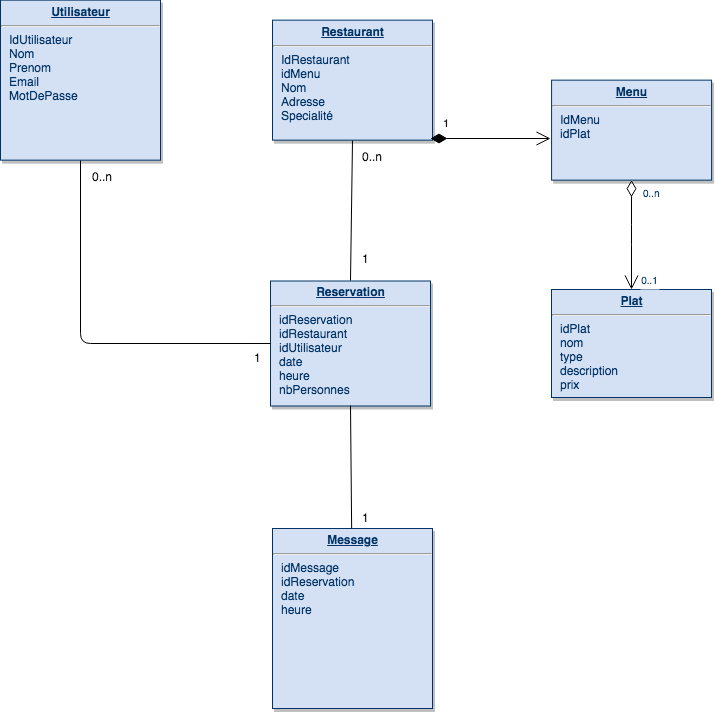
\includegraphics[width=\textwidth]{images/er1.png}
            \caption{Diagramme entité/association de notre cas}
        \end{figure}
        Si nous comparons ce diagramme à notre grille d'exigences, nous notons qu'il permet d'exprimer des exigences fonctionnelles mais de façon incomplète. En effet, dans ce diagramme, il n'y a aucune précision quant à comment se connecter, sur les conditions d'annulation, sur la façon dont le restaurant doit recevoir sa réservation, etc. De plus, ce diagramme est facilement lisible par tout le monde, et le temps d'apprentissage pour produire ce type de diagramme semble acceptable au vu de sa simplicité. Toutefois, ce type de diagramme ne permet pas de générer des tests et les représentations graphiques proposées ne sont pas orientées domaine. 

        \begin{table}[H]
        \centering
             \begin{tabular}{|p{25em}|p{5em}|} 
             \hline
            Critère & Répond au critère \\ [0.5ex] 
             \hline
             La modélisation doit pouvoir exprimer l’exigence & \cellcolor[HTML]{D03737}NON\\
             \hline
            La modélisation doit être lisible par n’importe quelle partie prenante & \cellcolor[HTML]{699A73}OUI\\
             \hline
            La modélisation doit pouvoir être écrite par les personnes qui expriment l’exigence &\cellcolor[HTML]{699A73} OUI \\
             \hline
            La modélisation doit permettre de générer des tests & \cellcolor[HTML]{D03737}NON \\
             \hline
            Les tests générés doivent être des tests fonctionnels &\cellcolor[HTML]{D03737} NON\\ 
             \hline
            N’importe quel domaine peut modéliser avec cet outil.&\cellcolor[HTML]{699A73} OUI\\ 
             \hline
            Le domaine est au coeur de la modélisations &\cellcolor[HTML]{D03737} NON\\ 
            \hline 
            \end{tabular}
            \caption{Évaluation du diagramme entité-association selon les critères défini}
            \end{table}

        \paragraph{Le diagramme de classe}
        
        Ce diagramme représente les classes et les interfaces ainsi que les relations entre elles. Une classe est représentée par un rectangle, possède des attributs, une visibilité, une multiplicité. Les classes peuvent hériter l'une de l'autre, s'agréger ou l'une peut composer l'autre.
    
        \begin{figure}[H]
            \centering
            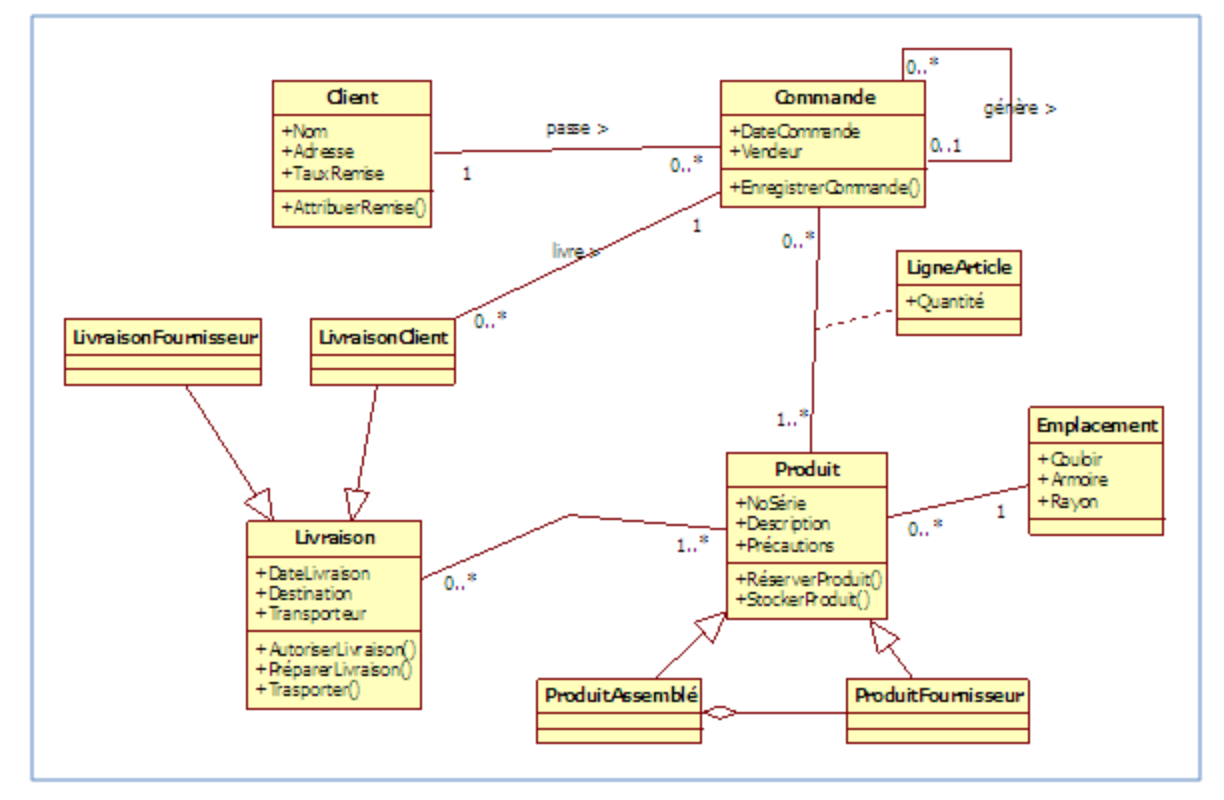
\includegraphics[width=\textwidth]{classe.png}
            \caption{Exemple de diagramme de classe}
        \end{figure}

        Bien que ce diagramme offre un niveau de détail plus important que le diagramme d'utilisation concernant le comportement de la solution, il reste toutefois que la notation n'a aucun lien avec le domaine. D'autre part, un diagramme de classe ne semble pas être simple pour toutes les parties prenantes. 

        \begin{table}[H]
        \centering
         \begin{tabular}{|p{25em}|p{5em}|} 
         \hline
        Critère & Répond au critère \\ [0.5ex] 
         \hline
         La modélisation doit pouvoir exprimer l’exigence & \cellcolor[HTML]{D03737}NON\\
         \hline
        La modélisation doit être lisible par n’importe quelle partie prenante & \cellcolor[HTML]{699A73}OUI\\
         \hline
        La modélisation doit pouvoir être écrite par les personnes qui expriment l’exigence &\cellcolor[HTML]{699A73} OUI \\
         \hline
        La modélisation doit permettre de générer des tests & \cellcolor[HTML]{D03737}NON \\
         \hline
        Les tests générés doivent être des tests fonctionnels &\cellcolor[HTML]{D03737} NON\\ 
         \hline
        N’importe quel domaine peut modéliser avec cet outil.&\cellcolor[HTML]{699A73} OUI\\ 
         \hline
        Le domaine est au coeur de la modélisations &\cellcolor[HTML]{D03737} NON\\ 
        \hline 
        \end{tabular}
        \caption{Évaluation du diagramme de classe selon les critères défini}
        \end{table}

        \paragraph{Les diagrammes de flux de données}

        Ce diagramme popularisé à la fin des années 1970 permet de représenter graphiquement comment l'information circule dans un processus ou un système.Ce type de diagramme est composé de :
         \begin{itemize}
            \item Flux de données avec des étiquettes 
            \item Des transformations de données (en cercle ou bulles) pour schématiser les processus
            \item Des magasins de données (lignes horizontales parallèles)
            \item Entités extérieures au système (rectangles)
        \end{itemize}

        \begin{figure}[H]
            \centering
            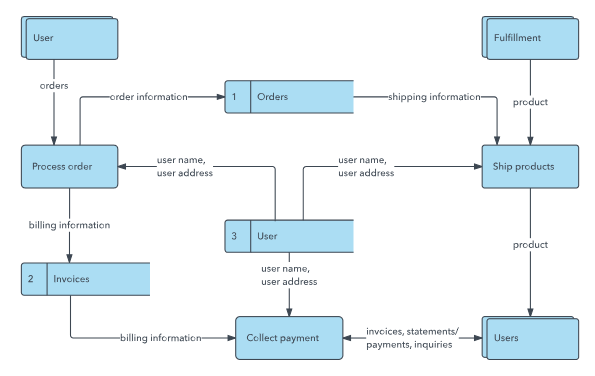
\includegraphics[width=\textwidth]{dataflow.PNG}
            \caption{Exemple de diagramme de flux de données}
        \end{figure}
    
         Les diagrammes de flux de donnée proposent des niveaux de détail numérotés 0, 1 ou 2 et vont parfois jusqu'à 3 ou plus.

        \textit{Niveau 0}
    
        Ce diagramme est appelé diagramme de contexte. Il représente une vue globale du système, montrant un processus unique de haut avec ses relations externes. Ce diagramme est généralement compréhensible par toutes les parties prenantes  mais de part son aspect général ne fournit pas assez de détails pour spécifier des tests d'acceptation. 
        \begin{figure}[H]
                \centering
                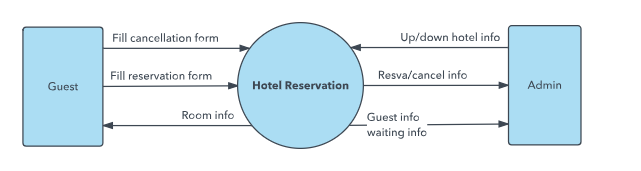
\includegraphics[width=\textwidth]{DFD1.PNG}
                \caption{Exemple de DFD de niveau 0}
            \end{figure}
            
        \textit{Niveau 1}

        Ce diagramme fournit des détails aux diagramme de context. Les fonctions principales du système sont mises en évidence. Le processus unique est découpé en sous processus.
    
        \begin{figure}[H]
            \centering
            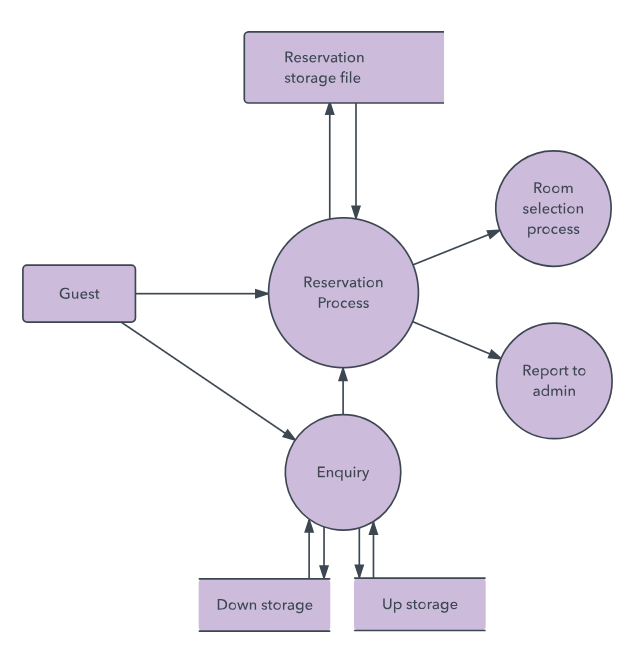
\includegraphics[width=\textwidth]{DFD2.PNG}
            \caption{Exemple de DFD de niveau 1}
        \end{figure}
        \textit{Niveau 2}
    
         Ce diagramme entre encore plus en détail dans la description des processus. 
    
        Les niveaux de détails 3 et 4 sont possibles à mettre en place mais restent assez rares. 
    
        Avec un diagramme assez détaillé, les développeurs peuvent l'utiliser pour commencer à rédiger du pseudocode. Un DFD peut fournir un bon point de départ pour modéliser les exigences mais lors du système réel, il n'est pas suffisant pour les testeurs. Les DFD sont même moins précis que le langage naturel pour les développeurs. Ce type de modélisation est intéressant pour visualiser les fonctions et les interfaces mais n'est pas suffisant pour éliciter correctement une exigence. \cite{livre4}

        \begin{table}[H]
        \centering
         \begin{tabular}{|p{25em}|p{5em}|} 
         \hline
        Critère & Répond au critère \\ [0.5ex] 
         \hline
         La modélisation doit pouvoir exprimer l’exigence & \cellcolor[HTML]{D03737}NON\\
         \hline
        La modélisation doit être lisible par n’importe quelle partie prenante & \cellcolor[HTML]{699A73}OUI\\
         \hline
        La modélisation doit pouvoir être écrite par les personnes qui expriment l’exigence &\cellcolor[HTML]{699A73} OUI \\
         \hline
        La modélisation doit permettre de générer des tests & \cellcolor[HTML]{D03737}NON \\
         \hline
        Les tests générés doivent être des tests fonctionnels &\cellcolor[HTML]{D03737} NON\\ 
         \hline
        N’importe quel domaine peut modéliser avec cet outil.&\cellcolor[HTML]{D03737} NON\\ 
         \hline
        Le domaine est au coeur de la modélisations &\cellcolor[HTML]{D03737} NON\\ 
        \hline 
        \end{tabular}
        \caption{Évaluation du diagramme de flux de données selon les critères défini}
        \end{table}

        Les modélisations qui représentent une vue beaucoup trop globale et seulement structurelle des exigences semblent ne pas être suffisantes pour remplir tous les critères que nous avons défini. Il semble également nécessaire de représenter le comportement des exigences, d'ajouter une partie dynamique à l'expression de ces exigences. 
        
        \subsubsection{Modélisation comportementale}

        \paragraph{Le diagramme de cas d'utilisation}

        Ce diagramme permet de décrire les différents acteurs du système et les fonctionnalités que chacun d'entre eux doit pouvoir réaliser. Chaque fonctionnalité est généralement représentée par un ovale dans lequel l'action est décrite. Les traits entre les acteurs et les cas d'utilisations sont des associations et/ou des inclusions. 

        \begin{figure}[H]
            \centering
            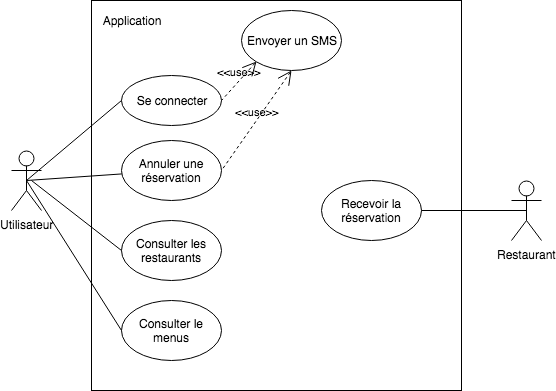
\includegraphics[width=\textwidth]{images/useeCAse.png}
            \caption{Diagramme de cas d'utilisation de notre cas}
        \end{figure}

        Ce diagramme permet d'avoir une vision très global de ce que doit pouvoir faire un acteur mais ne prend pas en compte les différents scénarios qui peuvent exister et qui peuvent être en eux même des exigences à spécifier.

        \begin{table}[H]
        \centering
         \begin{tabular}{|p{25em}|p{5em}|} 
         \hline
        Critère & Répond au critère \\ [0.5ex] 
         \hline
         La modélisation doit pouvoir exprimer l’exigence & \cellcolor[HTML]{D03737}NON\\
         \hline
        La modélisation doit être lisible par n’importe quelle partie prenante & \cellcolor[HTML]{699A73}OUI\\
         \hline
        La modélisation doit pouvoir être écrite par les personnes qui expriment l’exigence &\cellcolor[HTML]{699A73} OUI \\
         \hline
        La modélisation doit permettre de générer des tests & \cellcolor[HTML]{D03737}NON \\
         \hline
        Les tests générés doivent être des tests fonctionnels &\cellcolor[HTML]{D03737} NON\\ 
         \hline
        N’importe quel domaine peut modéliser avec cet outil.&\cellcolor[HTML]{699A73} OUI\\ 
         \hline
        Le domaine est au coeur de la modélisations &\cellcolor[HTML]{D03737} NON\\ 
        \hline 
        \end{tabular}
        \caption{Évaluation du diagramme d'utilisation selon les critères défini}
        \end{table}
    
        \paragraph{Le scénario}

        Le scénario est une description textuelle d'un cas d'utilisation. Décrire un cas d'utilisation permet notamment de déterminer quelle action arrive avant ou après une autre action, de bien comprendre comment la fonctionnalité doit se dérouler ou encore de connaître les contraintes relatives à ce cas. Un scénario est représenté par une fiche descriptive composé de l'identification, de la description du scénario, la et les post-conditions et les compléments. 
        \begin{figure}[H]
            \centering
            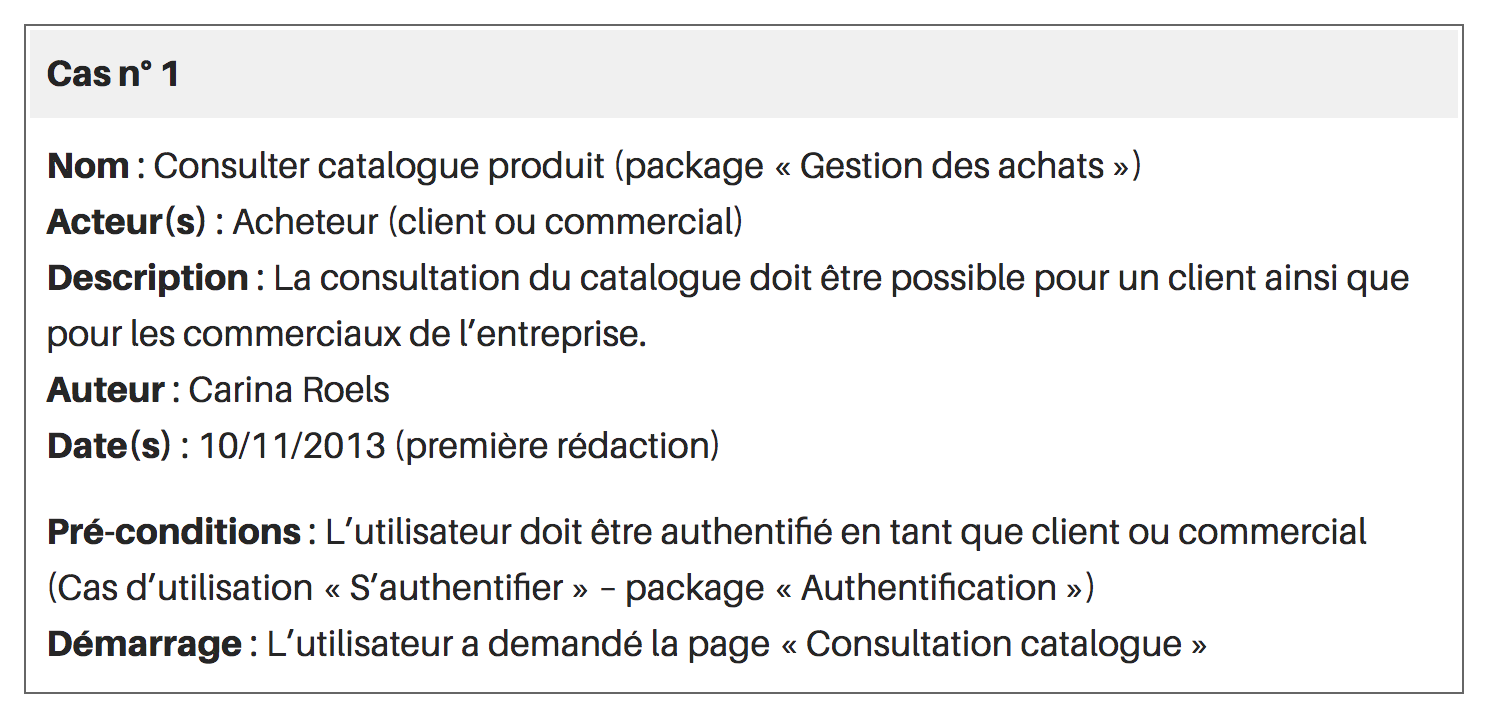
\includegraphics[width=\textwidth]{scenar.png}
            \caption{Exemple de fiche descriptive d'une scénario}
        \end{figure}
        
        Avec ce type de fiches descriptive que l'on peut standardiser, nous avons un début de formalisme d'une exigence. Toutefois, la description de l'exigence reste purement textuelle. Il est donc compliqué à partir de cette fiche de générer entièrement un test. Il existe une façon plus schématique et moins textuel de représenter un scénario : le diagramme de séquence.
        \begin{table}[H]
        \centering
         \begin{tabular}{|p{25em}|p{5em}|} 
         \hline
        Critère & Répond au critère \\ [0.5ex] 
         \hline
         La modélisation doit pouvoir exprimer l’exigence & \cellcolor[HTML]{699A73}OUI\\
         \hline
        La modélisation doit être lisible par n’importe quelle partie prenante & \cellcolor[HTML]{699A73}OUI\\
         \hline
        La modélisation doit pouvoir être écrite par les personnes qui expriment l’exigence &\cellcolor[HTML]{699A73} OUI \\
         \hline
        La modélisation doit permettre de générer des tests & \cellcolor[HTML]{D03737}NON \\
         \hline
        Les tests générés doivent être des tests fonctionnels &\cellcolor[HTML]{D03737} NON\\ 
         \hline
        N’importe quel domaine peut modéliser avec cet outil.&\cellcolor[HTML]{699A73} OUI\\ 
         \hline
        Le domaine est au coeur de la modélisations &\cellcolor[HTML]{699A73} OUI\\ 
        \hline 
        \end{tabular}
        \caption{Évaluation du scénario selon les critères défini}
        \end{table}
    
        \paragraph{Le diagramme de séquence}

        Le diagramme de séquence permet de décrire de façon détaillée les interactions entre les différentes instances du système pour un scénario d'utilisation donné. 
        
            \begin{figure}[H]
                \centering
                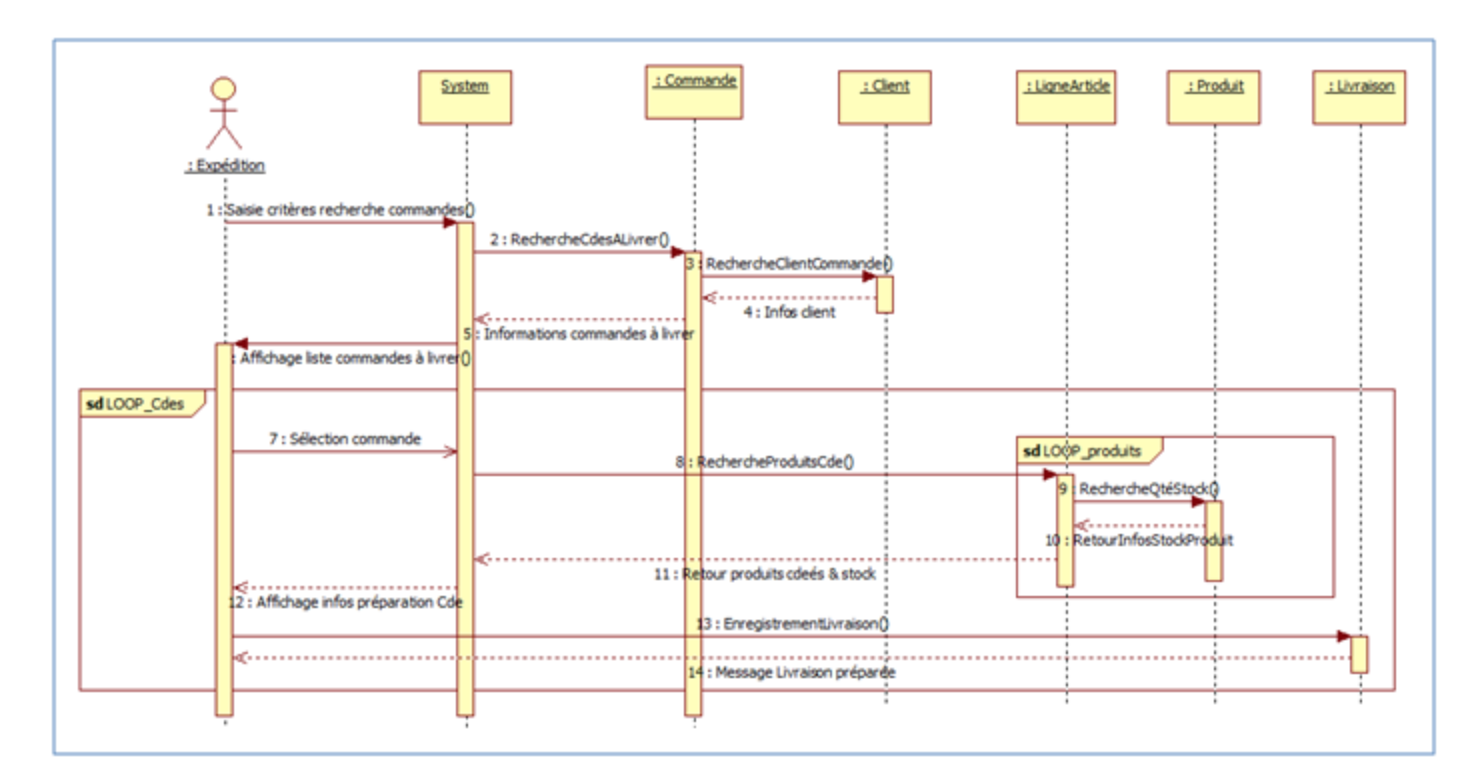
\includegraphics[width=\textwidth]{sequence.png}
                \caption{Exemple de diagramme de séquence}
            \end{figure}
        
        Il existe plusieurs approches qui ont été développées dans plusieurs articles de recherches pour générer et dériver des cas de tests à partir d'un diagramme de séquence.~\cite{article8, article9}

        \begin{table}[H]
        \centering
         \begin{tabular}{|p{25em}|p{5em}|} 
         \hline
        Critère & Répond au critère \\ [0.5ex] 
         \hline
         La modélisation doit pouvoir exprimer l’exigence & \cellcolor[HTML]{699A73}OUI\\
         \hline
        La modélisation doit être lisible par n’importe quelle partie prenante & \cellcolor[HTML]{D03737}NON\\
         \hline
        La modélisation doit pouvoir être écrite par les personnes qui expriment l’exigence &\cellcolor[HTML]{D03737} NON \\
         \hline
        La modélisation doit permettre de générer des tests & \cellcolor[HTML]{699A73}OUI \\
         \hline
        Les tests générés doivent être des tests fonctionnels &\cellcolor[HTML]{699A73} OUI\\ 
         \hline
        N’importe quel domaine peut modéliser avec cet outil.&\cellcolor[HTML]{699A73} OUI\\ 
         \hline
        Le domaine est au coeur de la modélisations &\cellcolor[HTML]{D03737} NON\\ 
        \hline 
        \end{tabular}
        \caption{Évaluation du diagramme de séquence selon les critères défini}
        \end{table}
    
        \paragraph{Le diagramme d'activité}

        Ce diagramme décrit le déroulement des différentes actions successives d'un système sans utiliser les objets ce qui permet plus de clarté pour les clients qui ont une vision domaine et non technique.
             \begin{figure}[H]
                \centering
                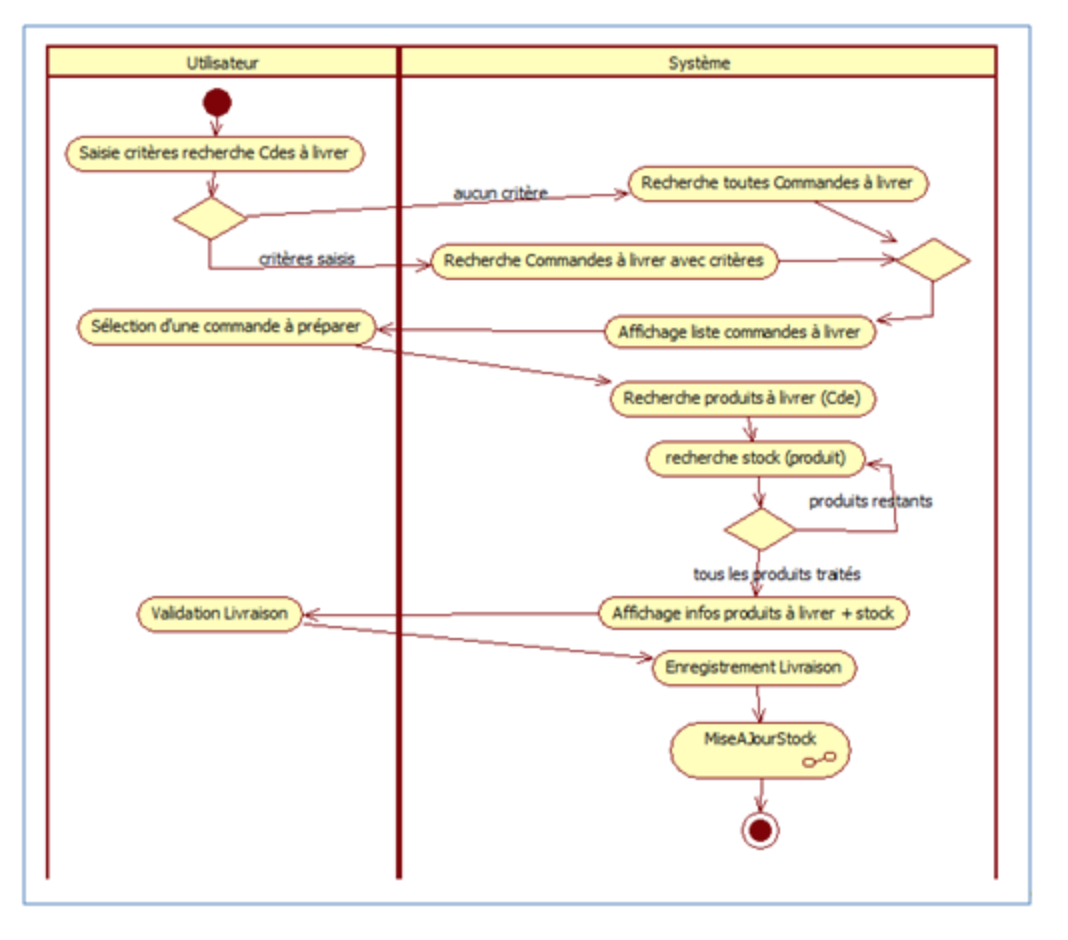
\includegraphics[width=\textwidth]{activite.png}
                \caption{Exemple de diagramme d'activité}
            \end{figure}
        Des approches ont également été proposées~\cite{article10} pour générer des cas de test à partir de ce types de diagrammes.
        \begin{table}[H]
        \centering
         \begin{tabular}{|p{25em}|p{5em}|} 
         \hline
        Critère & Répond au critère \\ [0.5ex] 
         \hline
         La modélisation doit pouvoir exprimer l’exigence & \cellcolor[HTML]{699A73}OUI\\
         \hline
        La modélisation doit être lisible par n’importe quelle partie prenante & \cellcolor[HTML]{699A73}OUI\\
         \hline
        La modélisation doit pouvoir être écrite par les personnes qui expriment l’exigence &\cellcolor[HTML]{D03737} NON \\
         \hline
        La modélisation doit permettre de générer des tests & \cellcolor[HTML]{699A73}OUI \\
         \hline
        Les tests générés doivent être des tests fonctionnels &\cellcolor[HTML]{699A73} OUI\\ 
         \hline
        N’importe quel domaine peut modéliser avec cet outil.&\cellcolor[HTML]{699A73} OUI\\ 
         \hline
        Le domaine est au coeur de la modélisations &\cellcolor[HTML]{D03737} NON\\ 
        \hline 
        \end{tabular}
        \caption{Évaluation du diagramme d'activité selon les critères défini}
        \end{table}
    
        \paragraph{SysML : le diagramme d'exigence}

        \textit{SysML doit permettre à des acteurs de corps de métiers différents de collaborer autour d'un modèle commun pour définir un système. }~\cite{sysml}.A l'instar d'UML, SysML est un langage constitué de plusieurs diagrammes. La majorité de ces derniers sont communs à UML. Par conséquent, nous présenterons dans cette sous partie que le diagramme d'exigences.Il s'agit d'un diagramme qui décrit les fonctions du logiciel. Il décrit les spécifications fonctionnelles.
    
         \begin{figure}[H]
            \centering
            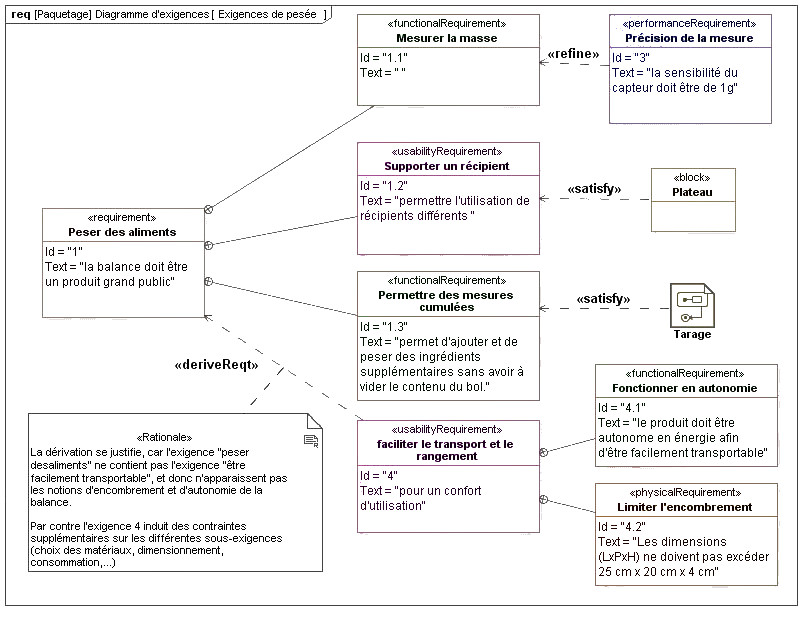
\includegraphics[width=\textwidth]{diagExi.jpg}
            \caption{Exemple de diagramme d'exigences~\cite{diagExi}}
        \end{figure}
    
        Bien qu'il soit possible d'importer ce diagramme dans des outils d'automatisation de test pour générer des scripts exécutables de test, il n'en reste pas moins que comme pour UML les spécificités du domaine et le langage utilisé n'est pas simple d'utilisation pour toutes les personnes impliquées dans le projet.
    
        \begin{table}[H]
        \centering
         \begin{tabular}{|p{25em}|p{5em}|} 
         \hline
        Critère & Répond au critère \\ [0.5ex] 
         \hline
         La modélisation doit pouvoir exprimer l’exigence & \cellcolor[HTML]{699A73}OUI\\
         \hline
        La modélisation doit être lisible par n’importe quelle partie prenante & \cellcolor[HTML]{D03737}NON\\
         \hline
        La modélisation doit pouvoir être écrite par les personnes qui expriment l’exigence &\cellcolor[HTML]{D03737} NON \\
         \hline
        La modélisation doit permettre de générer des tests & \cellcolor[HTML]{699A73}OUI \\
         \hline
        Les tests générés doivent être des tests fonctionnels &\cellcolor[HTML]{699A73} OUI\\ 
         \hline
        N’importe quel domaine peut modéliser avec cet outil.&\cellcolor[HTML]{699A73} OUI\\ 
         \hline
        Le domaine est au coeur de la modélisations &\cellcolor[HTML]{D03737} NON\\ 
        \hline 
        \end{tabular}
        \caption{Évaluation du diagramme d'exigences selon les critères défini}
        \end{table}
        
        \subsubsection{Les méthodes formelles}
        
        \paragraph{Les Réseaux de Petri}
        
        \textit{\guillemotleft Les réseaux de Pétri sont un outil graphique et mathématique qui s’applique à un grand nombre de domaine où les notions d’évènements et d’évolutions simultanées sont importantes\guillemotright}~\cite{article14} Avec ce type de modélisation il est possible de générer des tests, notamment à partir des réseaux de pétri haut niveau comme les modèles de test~\cite{article15}. Bien que des tests puissent être générés ce type de modélisation est difficilement lisible et difficile à écrire pour les experts métier notamment. 
        
        \paragraph{La méthode B}
        
        La méthode B permet de modéliser les spécifications de manière  abstraite. A l'instar des réseaux de Pétri, cette modélisation est beaucoup trop complexes pour les différentes parties prenantes.
        
        Malgré la possibilité à partir des méthodes formelles de générer des cas de tests, il n'en reste pas moins que ces méthodes ne sont pas adapté à la compréhension de tous.
    
        \subsubsection{Les Domain Specific Languages}

        Au delà de la capacité pour un type de modélisation à générer des tests, il important que toutes les exigences fonctionnelles puissent être correctement modélisées. Nous avons vu que les modélisations comme UML ou encore les diagrammes de flux permettent d'avoir une vision globale et/ou détaillée des exigences. Toutefois, le formalisme de ces diagrammes imposent des notations, des abstractions et conception. Or, certains domaines nécessitent une flexibilité quant à l'expression des exigences fonctionnelles. De plus, ces modélisations sont souvent pas les meilleures pour les utilisateurs finaux désirant une notation plus familière~\cite{article3}. En effet, UML peut être difficile à appréhender pour les clients. Cette sous partie présente les DSL qui sont des langages de modélisations spécifiques à un domaine. Avec ces langages déclaratifs~\cite{article4} il est possible d'une part de fournir des abstractions au niveau du domaine et d'autre part de permettre aux clients d'exprimer les exigences avec un langage dédié à leur domaine qui leur est compréhensible.
    
    
        \textit{Un langage spécifique au domaine (DSL) est un langage de programmation ou un langage de spécification exécutable qui offre, par des notations et des abstractions appropriées, un pouvoir expressif axé sur, et généralement restreint à, un domaine particulier de problème}~\cite{article4}.
    
        Les DSL ont de nombreux avantages pour la modélisation des exigences. Tout d'abord ils permettent une facilité d'utilisation et une meilleure expressivité par rapport aux modélisations à usage général. Ils permettent aux experts domaine de comprendre, valider, modifier et même parfois programmer les programmes~\cite{article4,article3}. Les DSL offrent également l'avantage d'écrire des exigences précises et indépendantes des plate formes~\cite{article3}.D'autre part, les DSL améliorent la testabilité en suivant des approches telles que citées dans~\cite{article11,article4}.Il existe des outils qui permettent à partir d'un DSL prédéfini de générer des tests d'acceptation. Ces outils et méthodes sont décrits dans la partie suivante.

    \subsection{De la modélisation vers les tests d'acceptation - Les framework BDD}

        \subsubsection{Cocumber}

        Cocumber est un outil qui permet de lancer automatiquement des tests d'acceptation et qui est créé en behaviour-driven developpement. Ce dernier est une méthode qui encourage la collaboration entre les différentes parties prenantes. L'outil est basé sur Gherkin qui est le format des spécifications Cocumber. Il est lisible par le client. Il s'agit d'un DSL qui permet à tout le monde de comprendre facilement le comportement attendu du logiciel. Pour définir une structure, Gherkin a des espaces et des indentations. 
        
        Quelques exemples de la synthaxe Gherkin : Feature, Background, Scenario, Given, When, Then,And,But,Scenario outline,Examples,Scenario Templates. Les fichiers rédigés pourront ensuite générer des signatures de méthodes. Les développeurs devront rédiger le corps de la méthode de test. 
        
            \begin{figure}[H]
                \centering
                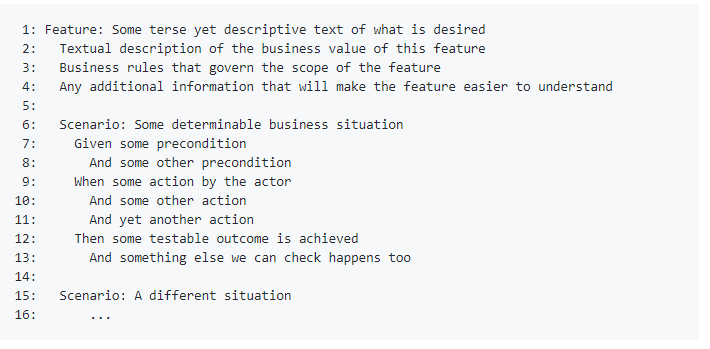
\includegraphics[width=\textwidth]{gherkinSyntax.PNG}
                \caption{Exemple de synthaxe Gherkin}
            \end{figure}
        
        Cocumber offre une réel avantage : celui de la génération de test à partir d'exigences rédigés dans un langage domaine. Toutefois, il n'existe pas de retour des tests vers les spécifications initiales.
        
        \subsubsection{EasyB}
        
        Cet outil est un framework basé sur Groovy qui utilise un langage DSL pour la plateforme Java. Groovy est utilisé pour exprimer les scnérarios.
            \begin{figure}[H]
                \centering
                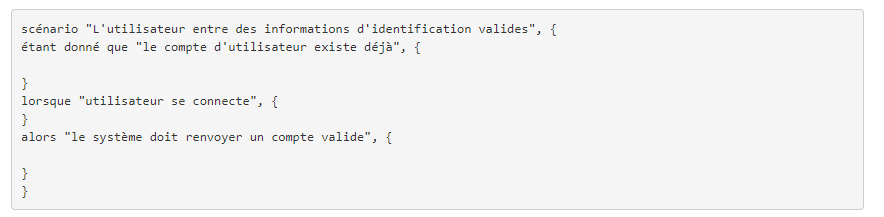
\includegraphics[width=\textwidth]{images/easyB.PNG}
                \caption{Exemple de scénario Groovy}
            \end{figure}
        
        Un rapport textuel de scénario est créé à la fin de chaque execution de tests. 
            
            \begin{figure}[H]
                \centering
                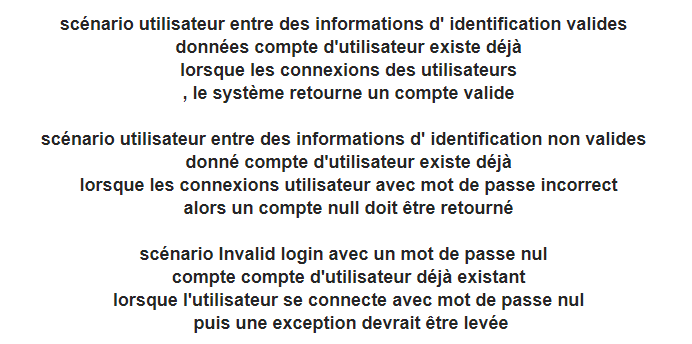
\includegraphics[width=\textwidth]{images/rapportEasyB.PNG}
                \caption{Exemple de rapport EasyB}
            \end{figure}
        
        \subsubsection{JDave}
        
        Jdave est un framework qui permet de spécifier le comportement des classes. Un comportement défini le comportement d'une classe selon un certain context. Cet outil nous parait beaucoup trop technique et intervient sur le code plutôt que sur les abstraction domaine. 
        
        \subsubsection{Concordion}
        Cet outil permet d'écrire des scripts d'automatisation des tests d'acceptation dans les projets basés sur JAVA. Les spécifications doivent être écrites en HTML. Ceci présente plusieurs inconvénients : l'expert métier doit savoir écrire du HTML et le langage HTML ne permet pas de décrire correctement les exigences.
        
        Ces deux derniers outils sont beaucoup trop spécifiques au langage de programmation.

        \subsubsection{Ravenflow - Bender RBY - Rational Rhapsody }
        
        Il existe des outils tel que Ravenflow qui permettent de générer des cas de tests à partir de formes d'exigences. Ce type d'outil se base sur des cas d'utilisation dans un format structuré et identifie chaque chemin à traver ces derniers. 
        
        Il existe également des outils plus rigoureux tel que Bender RBT qui développe des flux logiques de graphes cause/effet à partir d'une méthode structurée de documentation des spécifications fonctionnelles et identifie l'ensemble minimum de tests.
        
        Les outils d'analyse d'état, tels que Rational Rhapsody, dessinent un diagramme d'état à partir de descriptions structurées des différents états d'une unité, qui peuvent être un périphérique ou un programme.L'état détermine les comportements que l'unité doit et ne doit pas présenter, y compris ce qui déclenche la transition vers un autre état spécifié. Les cas de test sont alors définis pour exercer chaque chemin d'états, démontrant les comportements qu'il devrait présenter et assurant que ceux qu'il ne devrait pas présenter ne se produisent pas.
    
    \subsection{Conclusion}
    Pour conclure, nous avons vu que les outils passant des exigences rédigées en langage naturel aux tests ne proposent pas de manière d'automatiser les tests d'acceptation. Nous avons donc ensuite présenté différentes façons de modéliser les exigences pour pouvoir dans un second temps générer des tests à partir de ceux-ci. Bien que les notations UMLs/SysML soient riches en diagrammes et proposent de la génération de code, il est nécessaire d'avoir une certaine connaissance en modélisation et les notions spécifiques d'un domaine peuvent être mal (ou pas du tout) représentées. Les Domain Specific Language semblent être une bonne alternative : ils proposent de mettre le domaine au coeur de la modélisation et d'en générer les tests. Les outils comme Cocumber montrent qu'il est possible à partir DSL orienté langage naturel de générer des tests. En effet, les scénarios sont modélisés à travers des DSL et permettent de générer des tests. Toutefois, nous souhaitons améliorer la phase de recette en proposant un retour des tests au niveau des exigences. Nous détaillerons cette solution dans le chapitre 2 de ce mémoire. 

%%% Local Variables: 
%%% mode: latex
%%% TeX-master: "isae-report-template"
%%% End: 